\section{Tooling}\label{sec:tooling}
This chapter describes the tools that we developed while designing an implementing algorithms for scalafmt.
These tools were indispensable in giving us confidence that our algorithms worked as intended.

\subsection{Heatmaps}
Section~\ref{sec:optimizations} introduces several extensions to algorithm~\ref{alg:bfsv1} that were required go get acceptable performance.
In general, the extensions involved eliminating search states.
To identify code patterns that triggered excessive search growth, we developed heatmaps.

Heatmaps are a visualization that displays which code regions are most frequently visited in the best-first search.
Figure~\ref{fig:heatmap} shows an example heatmap.
\begin{figure}
  \centering
  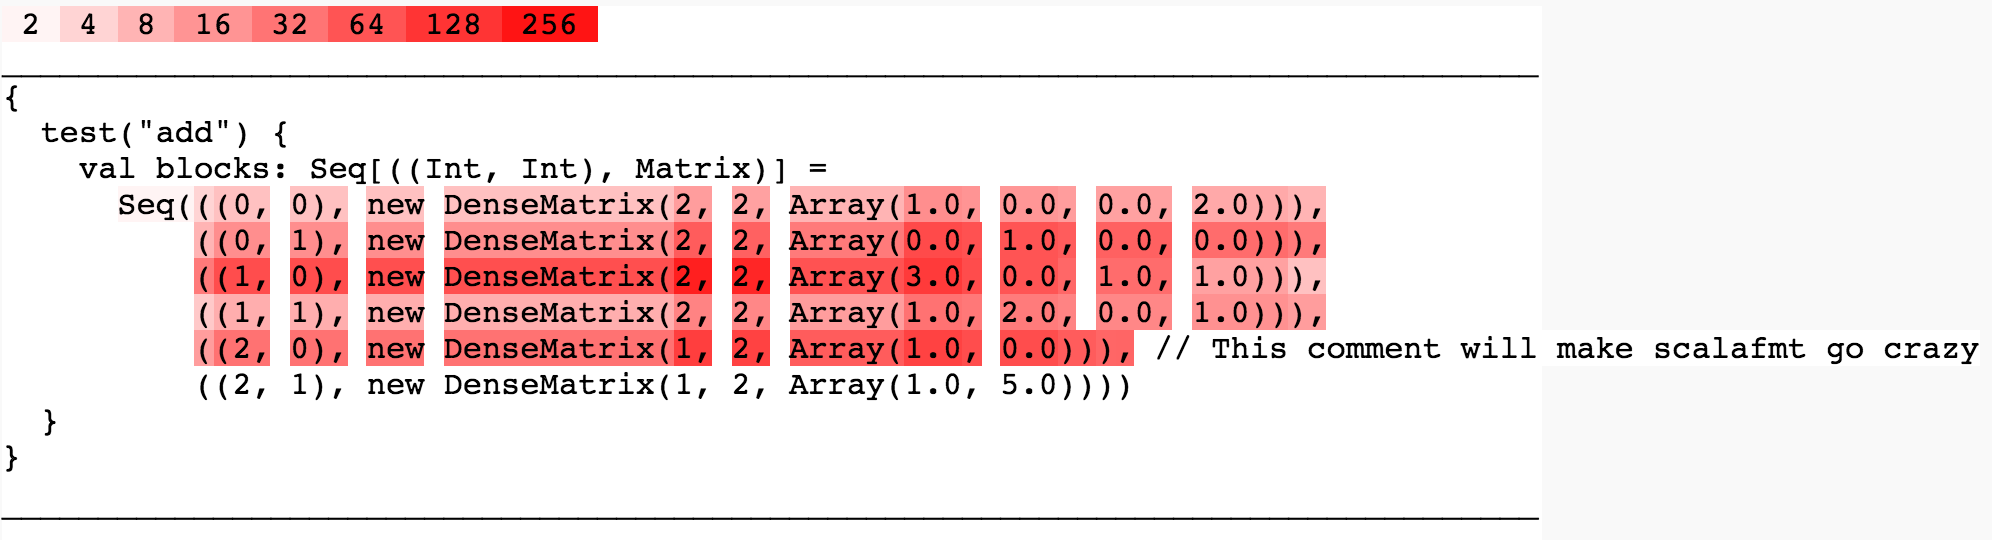
\includegraphics[width=\textwidth]{img/heatmap.png}
  \caption{Example heatmap with 5.121 visisted states}
  \label{fig:heatmap}
\end{figure}
The intensity of the red color indicates how often a particular token was visited.
A token highlighted by the lightest shade of red was visited twice while a token highlighted by the darkest shade of red was visited over 256 times.
This figure demonstrates several of the optimizations discussed in section~\ref{sec:optimizations}.
Firstly, thanks to the \texttt{dequeueOnNewStatements} optimization, the background is plain white up to the \texttt{Seq}.
The \texttt{Seq} gets visited twice, once when there's a space after the \texttt{=} and once when there's a newline.
Secondly, due to the OptimalToken optimization, when the search gets into trouble it backtracks to the tuple \texttt{(0, 0)} instead of the \texttt{Seq[((Int, Int), Matri)]} type signature.
Finally, because of the strategically placed comment at the end that exceeds the column limit, the search space grows out of bounds on the fourth argument triggering the \texttt{escapeInPathologicalCases} best-effort fallback.
Without heatmaps, it would be a much greater challenge to get these insights.
However, these heatmaps gave us limited insights in how our changes affected the search space in the best-first search.

We developed an extension to heatmaps that allows us to visually compare the difference in search space between two versions of scalafmt.
Figure~\ref{fig:heatmap2} shows an example of such a diff report.
\begin{figure}
  \centering
  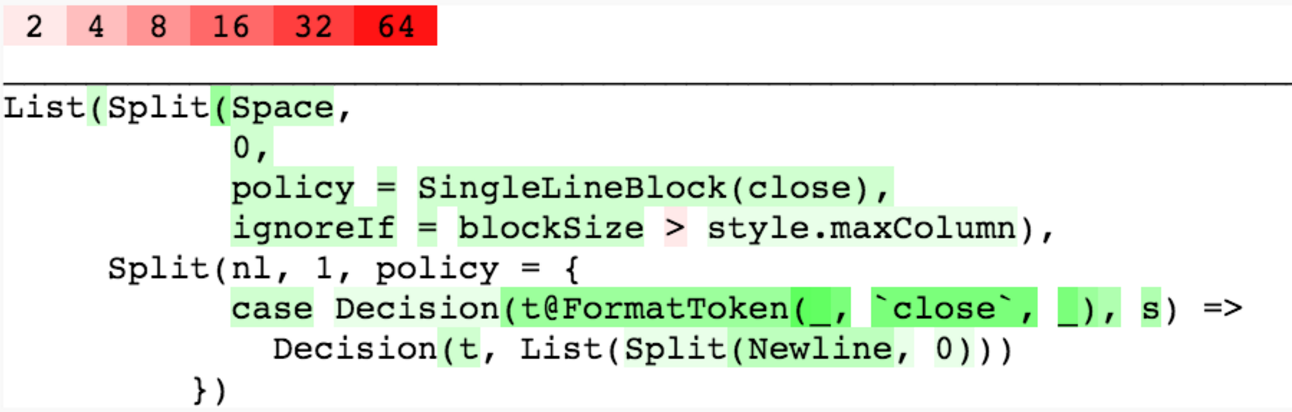
\includegraphics[width=\textwidth]{img/heatmap2.png}
  \caption{Example diff heatmap}
  \label{fig:heatmap2}
\end{figure}
The green background indicates that the new version of scalafmt makes fewer visits to those regions.
Observe that the \texttt{>} operator has a background with a light shade of red.
This means that the operator was visisted more often in the new scalafmt version.
A price well worth paying considering the overall shrink in search space.
To produce diff heatmaps, we first persist to a database the statistics report needed to generate a single heatmap after each test run.
Then, we generate the diff heatmap by fetching two reports and calculating the difference in visits per token.
If the difference is negative for a particular token --- meaning we visited said token fewer times --- the background is highlighted green, otherwise red.






\subsection{Traceability}\label{sec:line}
\subsection{Configuration}
\subsubsection{maxColumn}
\subsubsection{binPacking}
\subsubsection{vertical alignment}
\subsection{Testing}~\label{sec:testing}
\subsection{Unit tests}
\subsection{Property based tests}
\subsubsection{AST Integrity}
\subsubsection{Idempotency}
\subsection{Regressions tests}
